\chapter{Rating by sorting into relative performance quantiles}
\label{sec:9}

\abstract*{ In this chapter, we apply order statistics for sorting a set $X$ of $n$ potential decision alternatives, evaluated on $m$ incommensurable performance criteria, into $q$ quantile equivalence classes. The sorting algorithm is based on pairwise outranking characteristics involving the quantile class limits observed on each criterion. Thus we may implement a weak ordering algorithm of complexity $O(nmq)$.
}

\abstract{ In this chapter, we apply order statistics for sorting a set $X$ of $n$ potential decision alternatives, evaluated on $m$ incommensurable performance criteria, into $q$ quantile equivalence classes. The sorting algorithm is based on pairwise outranking characteristics involving the quantile class limits observed on each criterion. Thus we may implement a weak ordering algorithm of complexity $O(nmq)$.
}

\section{Quantile sorting on a single performance criterion}
\label{sec:9.1}

A single criterion sorting category $K$ is a (usually) lower-closed interval $[m_k ; M_k[$ on a real-valued performance measurement scale, with $m_k \leq M_k$. If $x$ is a measured performance on this scale, we may distinguish three sorting situations:
\begin{enumerate}[leftmargin=1cm,rightmargin=0.5cm,topsep=1pt]
\item $x < m_k$ and $x < M_k$: The performance $x$ is lower than category $K$.
\item $x \geqslant m_k$ and $x < M_k$: The performance $x$ belongs to category $K$.
\item $x > m_k$ and $x \geqslant M_k$: The performance $x$ is higher than category $K$.
\end{enumerate}

As the relation $<$ is the dual of $\geqslant$ ($\not\geqslant$), it will be sufficient to check that $x \geqslant m_k$ as well as $x \not\geqslant M_k$ are true for $x$ to be considered a member of category $K$.

Upper-closed categories (in a more mathematical integration style) may as well be considered. In this case it is sufficient to check that $m_k \not\geqslant x$ as well as $M_k \geqslant x$ are true for $x$ to be considered a member of category $K$. It is worthwhile noticing that a category $K$ such that $m_k = M_k$ is hence always empty by definition. In order to be able to properly sort over the complete range of values to be sorted, we will need to use a special, two-sided closed last, respectively first, category.

Let $K = {K_1 , ..., K_q}$ be a non trivial partition of the criterion’s performance measurement scale into $q \geq 2$ ordered categories $K_k$ – i.e. lower-closed intervals $[m_k ; M_k[$ – such that $m_k < M_k$, $M_k = m_{k+1}$ for $k = 0, ..., q - 1$ and $M_q = \infty$. And, let $A=\{a_1 , a_2 , a_3 , ...\}$ be a finite set of not all equal performance measures observed on the scale in question.

\textbf{Property}: For all performance measure $x \in A$ there exists now a unique $k$ such that $x \in K_k$. If we assimilate, like in descriptive statistics, all the measures gathered in a category $K_k$ to the central value of the category – i.e. $(m_k + M_k)/2$ – the sorting result will hence define a weak order (complete preorder) on $A$.

Let $Q=\{Q_0 , Q_1 , ..., Q_q\}$ denote the set of $q + 1$ increasing order-statistical quantiles –like quartiles or deciles– we may compute from the ordered set $A$ of performance measures observed on a performance scale. If $Q_0 = \min(X)$, the following intervals: $[Q_0 ; Q_1 [$, $[Q_1 ; Q_2 [$, ..., $[Q_{q-1}; \infty[$ define a set of $q$ lower-closed sorting categories. And, in the case of upper-closed categories, if $Q_q = \max(X)$, we obtain the intervals $] -\infty; Q_1]$, $]Q_1 ; Q_2]$, ..., $]Q_{q-1} ; Q_q]$. The corresponding sorting of $A$ will result, in both cases, in a repartition of all measures $x$ into the $q$ quantile categories $K_k$ for $k = 1, ..., q$.

\textbf{Example}: Let $A$ = \{ $a_7 = 7.03$, $a_{15}=9.45$, $a_{11}= 20.35$, $a_{16}= 25.94$, $a_{10}= 31.44$, $a_9= 34.48$, $a_{12}= 34.50$, $a_{13}= 35.61$, $a_{14}= 36.54$, $a_{19}= 42.83$, $a_5= 50.04$, $a_2= 59.85$, $a_{17}= 61.35$, $a_{18}= 61.61$, $a_3= 76.91$, $a_6= 91.39$, $a_1= 91.79$, $a_4= 96.52$, $a_8= 96.56$, $a_{20}= 98.42$ \} be a set of 20 increasing performance measures observed on a given criterion. The lower-closed category limits we obtain with quartiles ($q = 4$) are: $Q_0 = 7.03$ = $a_7$, $Q_1= 34.485$, $Q_2= 54.945$ (median performance), and $Q_3= 91.69$. And the sorting into these four categories defines on $A$ a complete preorder with the following four equivalence classes: $K_1=\{a_7,a_{10},a_{11},a_{10},a_{15},a_{16}\}$, $K_2=\{a_5,a_9,a_{13},a_{14},a_{19}\}$, $K_3=\{a_2,a_3,a_6,a_{17},a_{18}\}$, and $K_4=\{a_1,a_4,a_8,a_{20}\}$.

\section{Sorting into quantiles with multiple performance criteria}
\label{sec:9.2}

Let us now suppose that we are given a performance tableau with a set $X$ of $n$ decision alternatives evaluated on a coherent family of $m$ performance criteria associated with the corresponding outranking relation $\succsim$ defined on $X$. We denote $x_j$ the performance of alternative $x$ observed on criterion $j$.

Suppose furthermore that we want to sort the decision alternatives into $q$ upper-closed quantile equivalence classes. We therefore consider a series : $k = k/q$ for $k = 0, ..., q$ of $q+1$ equally spaced quantiles, like quartiles: $0$, $0.25$, $0.5$, $0.75$, $1$; quintiles: $0$, $0.2$, $0.4$, $0.6$, $0.8$, $1$: or deciles: $0$, $0.1$, $0.2$, ..., $0.9$, $1$, for instance.

The upper-closed $\mathbf{q}^k$ class corresponds to the m quantile intervals $]q_j(p_{k-1});q_j(p_k)]$ observed on each criterion $j$,  where $k = 2, ..., q$ , $q_j(p_q) =  \max_X(x_j)$, and the first class gathers all performances below or equal to $Q_j(p_1)$.

The lower-closed $\mathbf{q}_k$ class corresponds to the $m$ quantile intervals $[q_j(p_{k-1});q_j(p_k)[$ observed on each criterion $j$, where $k = 1, ..., q-1$, $q_j(p_0) = \min_X(x_j)$, and the last class gathers all performances above or equal to $Q_j(p_{q-1})$.

We call \textbf{q-tiles} a complete series of $k = 1, ..., q$ upper-closed $\mathbf{q}^k$, respectively lower-closed $\mathbf{q}_k$, multiple-criteria quantile classes.

\textbf{Property}: With the help of the bipolar-valued characteristic of the outranking relation $r(x \succsim y)$ we may compute as follws the bipolar-valued characteristic of the assertion: $x$ belongs to upper-closed $q$-tiles class $\mathbf{q}^k$ class, resp. lower-closed class $\mathbf{q}_k$ \citep{ADT-L10}:
\begin{eqnarray}\label{eq:9.1}
r(x \in \mathbf{q}^k) \; = \; \min \big[ -r\big(\mathbf{q}(p_{q-1}) \succsim x\big), \,r\big(\mathbf{q}(p_{q}) \succsim x)\big]\\
r(x \in \mathbf{q}_k) \; = \; \min \big[ r\big(x \succsim \mathbf{q}(p_{q-1})\big),\, -r\big(x \succsim\mathbf{q}(p_{q})\big)\big]
\end{eqnarray}

The \texttt{min} operator inplements the logical conjunction and, the outranking relation $\succsim$ verifying the coduality principle, $-r\big(\mathbf{q}(p_{q-1}) \succsim x\big) \,=\, r\big(\mathbf{q}(p_{q-1}) \prec x\big)$, resp. $-r\big(x \succsim \mathbf{q}(p_{q}) \,=\, r\big(x \prec \mathbf{q}(p_{q}\big)$.

The \texttt{QuantilesSortingDigraph} class \index{QuantilesSortingDigraph@\texttt{QuantilesSortingDigraph} class} from the \texttt{sortingDigraphs} module\index{sortingDigraphs@\texttt{sortingDigraphs} module} can compute, for instance, such a quintiling of a given random performance tableau \citep{BIS-2021b}.
\begin{lstlisting}[caption={Computing a quintiles sorting result},label=list:9.1,basicstyle=\ttfamily\scriptsize]
>>> from randomPerfTabs import RandomPerformanceTableau
>>> t = RandomPerformanceTableau(numberOfActions=50,seed=5)
>>> from sortingDigraphs import QuantilesSortingDigraph
>>> qs = QuantilesSortingDigraph(t,limitingQuantiles=5)
>>> qs
    *-----  Object instance description -----------*
     Instance class  : QuantilesSortingDigraph
     Instance name   : sorting_with_5-tile_limits
     Actions         : 50
     Criteria        : 7
     Categories      : 5
     Lowerclosed     : False
     Size            : 841
     Valuation domain  : [-1.00;1.00]
     Determinateness (%) : 81.39 §\label{line:9.1.15}§
     Attributes          : ['actions','actionsOrig',
          'criteria','evaluation','runTimes','name',
	  'limitingQuantiles','LowerClosed',
	  'categories','criteriaCategoryLimits',
	  'profiles','profileLimits','hasNoVeto',
	  'valuationdomain','nbrThreads','relation',
	  'categoryContent','order','gamma','notGamma']
     *------  Constructor run times (in sec.) ------*
     # Threads        : 1
     Total time       : 0.03120
     Data input       : 0.00300
     Compute profiles : 0.00075
     Compute relation : 0.02581
     Weak Ordering    : 0.00052
\end{lstlisting}

5-tiling the 50 decision alternatives results in 5 ordered upper-closed categories of decision alternatives --the quintiles-- supported by a $81.39\%$ majority of criteria significance (see Line~\ref{line:9.1.15} above).

The \texttt{showCriteriaQuantileLimits()}\index{showCriteriaQuantileLimits@\texttt{showCriteriaQuantileLimits()}} method shows in Listing~\vref{list:9.2} the quintile limits separating on each criterion the respective evaluations of the 50 decision alternatives into the 5 quintiles. Highest evaluations are observed on criterion \texttt{g1} (see Line~\ref{line:9.2.6} below). 
\begin{lstlisting}[caption={Inspecting the quantile limits},label=list:9.2]
>>> qs.showCriteriaQuantileLimits()
     Quantile Class Limits (q = 5)
     Upper-closed classes
     crit.	 0.20	 0.40	 0.60	 0.80	 1.00	 
     *------------------------------------------------
      g1	 31.35	 41.09	 58.53	 71.91	 98.08	 §\label{line:9.2.6}§
      g2	 27.81	 39.19	 49.87	 61.66	 96.18	 
      g3	 25.10	 34.78	 49.45	 63.97	 92.59	 
      g4	 24.61	 37.91	 53.91	 71.02	 89.84	 
      g5	 26.94	 36.43	 52.16	 72.52	 96.25	 
      g6	 23.94	 44.06	 54.92	 67.34	 95.97	 
      g7	 30.94	 47.40	 55.46	 69.04	 97.10
\end{lstlisting}

And with the \texttt{showSorting()}\index{showSorting@\texttt{showSorting()}} method we can inspect the actual quintiles sorting result in Listing~\ref{list:9.3} below.
\begin{lstlisting}[caption={Computing a quintiles sorting result},label=list:9.3]
>>> qs.showSorting()
    *--- Sorting results in descending order ---*
     ]0.80 - 1.00]: ['a22']
     ]0.60 - 0.80]: ['a03','a07','a08','a11','a14','a17',
                     'a19','a20','a29','a32','a33','a37',
		     'a39','a41','a42','a49']
     ]0.40 - 0.60]: ['a01','a02','a04','a05','a06','a08',
                     'a09','a16','a17','a18','a19','a21',
		     'a24','a27','a28','a30','a31','a35',
		     'a36','a40','a43','a46','a47','a48',
		     'a49','a50']
     ]0.20 - 0.40]: ['a04','a10','a12','a13','a15','a23',
                     'a25','a26','a34','a38','a43','a44',
		     'a45','a49']
     ]   < - 0.20]: ['a44']
   \end{lstlisting}

Most of the decision alternatives (26) are gathered in the median quintile $]0.40 - 0.60]$ class, whereas the highest quintile $]0.80-1.00]$ and the lowest quintile $]< - 0.20]$ classes gather each one a unique decision alternative (\texttt{a22}, resp. \texttt{a44}).

Inspecting the details of the corresponding sorting characteristics may be done with the \texttt{showSortingCharacteristics()} method\index{showSortingCharacteristics@\texttt{showSortingCharacteristics()}}.
\begin{lstlisting}[caption={Bipolar-valued sorting characteristics (extract)},label=list:9.4,basicstyle=\ttfamily\scriptsize]
>>> qs.showSortingCharacteristics()
     x  in  q^k          r(q^k-1 < x)  r(q^k >= x)  r(x in q^k)
    a22 in ]< - 0.20]	    1.00	 -0.86	      -0.86
    a22 in ]0.20 - 0.40]    0.86	 -0.71	      -0.71
    a22 in ]0.40 - 0.60]    0.71	 -0.71	      -0.71
    a22 in ]0.60 - 0.80]    0.71	 -0.14	      -0.14
    a22 in ]0.80 - 1.00]    0.14	  1.00	       0.14 §\label{line:9.4.7}§
    ...
    ...
    a44 in ]< - 0.20]	    1.00	  0.00	       0.00 §\label{line:9.4.10}§
    a44 in ]0.20 - 0.40]    0.00	  0.57	       0.00 §\label{line:9.4.11}§
    a44 in ]0.40 - 0.60]   -0.57	  0.86	      -0.57
    a44 in ]0.60 - 0.80]   -0.86	  0.86	      -0.86
    a44 in ]0.80 - 1.00]   -0.86	  0.86	      -0.86
    ...
    ...
    a49 in ]< - 0.20]	    1.00	 -0.43	      -0.43
    a49 in ]0.20 - 0.40]    0.43	  0.00	       0.00 §\label{line:9.4.18}§
    a49 in ]0.40 - 0.60]    0.00	  0.00	       0.00
    a49 in ]0.60 - 0.80]    0.00	  0.57	       0.00 §\label{line:9.4.20}§
    a49 in ]0.80 - 1.00]   -0.57	  0.86	      -0.57
\end{lstlisting}

In Listing~\vref{list:9.4} Line~\ref{line:9.4.7}, alternative \texttt{a22} verifies indeed positively both sorting conditions only for the highest quintile $[0.80 - 1.00]$ class. Whereas alternatives \texttt{a44} and \texttt{a49}, for instance, weakly verify both sorting conditions for two, resp. three, adjacent quintile classes (Lines~\ref{line:9.4.10}~-\ref{line:9.4.11} and \ref{line:9.4.18}-\ref{line:9.4.20}).  

Quantiles sorting results, indeed, verify always the following properties \citep{ADT-L10}:
\begin{property}[Formal properties of a quantiles sorting result]\label{prop:9.1}
\begin{enumerate}[leftmargin=0.5cm,rightmargin=0.5cm,topsep=1pt]
\item \emph{Coherence}: Each object is sorted into a non-empty subset of \emph{adjacent} $q$-tiles classes. An alternative that would \emph{miss} evaluations on all the criteria will be sorted conjointly in all $q$-tiled classes.
\item \emph{Uniqueness}: When $r(x \in \mathbf{q}^k) \neq 0.0$  for $k = 1, ..., q$, the performance $x$ is sorted into \emph{exactly one single} $q$-tiled class.
\item \emph{Separability}: Computing the sorting result for performance $x$ is \emph{independent} from the computing of the other performances’ sorting results. This property gives access to efficient parallel processing of class membership characteristics.
\end{enumerate}
\end{property}

The $q$-tiles sorting result leaves us hence with more or less \emph{overlapping} ordered quantile equivalence classes. For constructing now a linearly ranked q-tiles partition of $X$ , we may apply three strategies:
\begin{enumerate}[leftmargin=0.5cm,rightmargin=0.5cm,topsep=1pt]
\item \emph{Average} (default): In decreasing lexicographic order of the average of the lower and upper quantile limits and the upper quantile class limit;
\item \emph{Optimistic}: In decreasing lexicographic order of the upper and lower quantile class limits;
\item \emph{Pessimistic}: In decreasing lexicographic order of the lower and upper quantile class limits;
\end{enumerate}
\begin{lstlisting}[caption={Weakly ranking the quintiles sorting result},label=list:9.5]
>>> qs.showQuantileOrdering(strategy='average')
    ]0.80-1.00] : ['a22']
    ]0.60-0.80] : ['a03','a07','a11','a14','a20','a29',
                   'a32','a33','a37','a39','a41','a42']
    ]0.40-0.80] : ['a08','a17','a19']
    ]0.20-0.80] : ['a49'] §\label{line:9.5.6}§
    ]0.40-0.60] : ['a01','a02','a05','a06','a09','a16',
                    'a18','a21','a24','a27','a28','a30',
		    'a31','a35','a36','a40','a46','a47',
		    'a48','a50']
    ]0.20-0.60] : ['a04','a43']
    ]0.20-0.40] : ['a10','a12','a13','a15','a23','a25',
                    'a26','a34','a38','a45']
    ]  < -0.40] : ['a44']
\end{lstlisting}

Following, for instance, the \emph{average} ranking strategy, we find confirmed in the weak ranking shown in Listing~\vref{list:9.5}  that alternative \texttt{a49}  is indeed sorted into three adjacent quintiles classes, namely $]0.20-0.80]$ and precedes the $]0.40-0.60]$ class, of same average of lower and upper limits (see Line~\ref{line:9.5.6}).

The \texttt{QuantilesSortingDigraph} class constructor models hence a linearly ordered decomposition of the corresponding bipolar-valued outranking digraph. This decomposition leads us to a new \emph{sparse pre-ranked} outranking digraph model.

\section{The sparse pre-ranked outranking digraph model}
\label{sec:9.3}

Following the methodological requirements of the outranking approach, a given outranking digraph is, necessarily associated with a corresponding performance tableau (see Chap.~\ref{sec:3}). And, we can use this associated performance tableau for linearly decomposing the set of potential decision alternatives into ordered quantiles equivalence classes by using the quantiles sorting algorithm seen in the previous Section. 

In the coding example shown in Listing~\vref{list:9.6} below, we generate, first a simple performance tableau of 75 decision alternatives and, secondly, construct with the \texttt{PreRankedOutrankingDigraph} class\index{PreRankedOutrankingDigraph@\texttt{PreRankedOutrankingDigraph} class} from \texttt{sparseOut\-rankingDi\-graphs} module\index{sparseOutrankingDigraphs@\texttt{sparseOutrankingDigraphs} module} the corresponding sparse outranking digraph called \texttt{prg}. Notice by the way in Line~\ref{line:9.6.3} the \texttt{BigData} flag used for generating a parsimoniously commented performance tableau \citep{BIS-2021b}.
\begin{lstlisting}[caption={Computing a \emph{pre-ranked} sparse outranking digraph},label=list:9.6]
>>> from randomPerfTabs import RandomPerformanceTableau
>>> tp = RandomPerformanceTableau(numberOfActions=75,\
...                    BigData=True,seed=100)  §\label{line:9.6.3}§
>>> from sparseOutrankingDigraphs import\
...          PreRankedOutrankingDigraph
>>> prg = PreRankedOutrankingDigraph(Tp,quantiles=5)
>>> prg
    *----- Object instance description ------*
     Instance class    : PreRankedOutrankingDigraph
     Instance name     : randomperftab_pr
     Actions           : 75
     Criteria          : 7
     Sorting by        : 5-Tiling
     Ordering strategy : average §\label{line:9.6.14}§
     Components        : 9
     Minimal order     : 1
     Maximal order     : 25
     Average order     : 8.3
     fill rate         : 20.432% §\label{line:9.6.19}§
     Attributes        : ['actions','criteria','evaluation','NA','name', §\label{line:9.6.20}§
         'order','runTimes','dimension','sortingParameters',
	 'valuationdomain','profiles','categories','sorting',
	 'decomposition','nbrComponents','components',
	 'fillRate','minimalComponentSize','maximalComponentSize',
              ... ]
\end{lstlisting}

The ordering of the 5-tiling result is following the \emph{average} lower and upper quintile limits strategy (see List.~\vref{list:9.6} Line~\ref{line:9.6.14}). We obtain here 9 ordered components of minimal order 1 and maximal order 25. With the \texttt{showDecomposition()} method\index{showDecomposition@\texttt{showDecomposition()}}, the corresponding \emph{pre-ranked decomposition} may be inspected as follows:
\begin{lstlisting}[caption={The quantiles decomposition of a pre-ranked outranking digraph},label=list:9.7]
>>> prg.showDecomposition()
    *--- quantiles decomposition in decreasing order---*
     c1. ]0.80-1.00] : [5, 42, 43, 47] §\label{line:9.7.3}§
     c2. ]0.60-1.00] : [73]
     c3. ]0.60-0.80] : [1, 4, 13, 14, 22, 32, 34, 35, 40,
                        41, 45, 61, 62, 65, 68, 70, 75]
     c4. ]0.40-0.80] : [2, 54]
     c5. ]0.40-0.60] : [3, 6, 7, 10, 15, 18, 19, 21, 23, 24,
                        27, 30, 36, 37, 48, 51, 52, 56, 58,
			63, 67, 69, 71, 72, 74]
     c6. ]0.20-0.60] : [8, 11, 25, 28, 64, 66]
     c7. ]0.20-0.40] : [12, 16, 17, 20, 26, 31, 33, 38, 39,
                        44, 46, 49, 50, 53, 55]
     c8. ]   <-0.40] : [9, 29, 60]
     c9. ]   <-0.20] : [57, 59] §\label{line:9.7.15}§
\end{lstlisting}

The highest quintile class ($]80\%-100\%]$) contains decision alternatives \texttt{5}, \texttt{42}, \texttt{43} and \texttt{47}. Lowest quintile class ($]-20\%]$) gathers alternatives \texttt{57} and \texttt{59} (see List.~\vref{list:9.7} Lines~\ref{line:9.7.3} and~\ref{line:9.7.15}).

The resulting sparse outranking relation is shown with the \texttt{showHTMLRela\-tionMap()} method\index{showHTMLRelationMap@\texttt{showHTMLRelationMap()}} in a heatmap browser view.
\begin{lstlisting}
   >>> prg.showHTMLRelationMap()
\end{lstlisting}
\begin{figure}[ht]
%\sidecaption
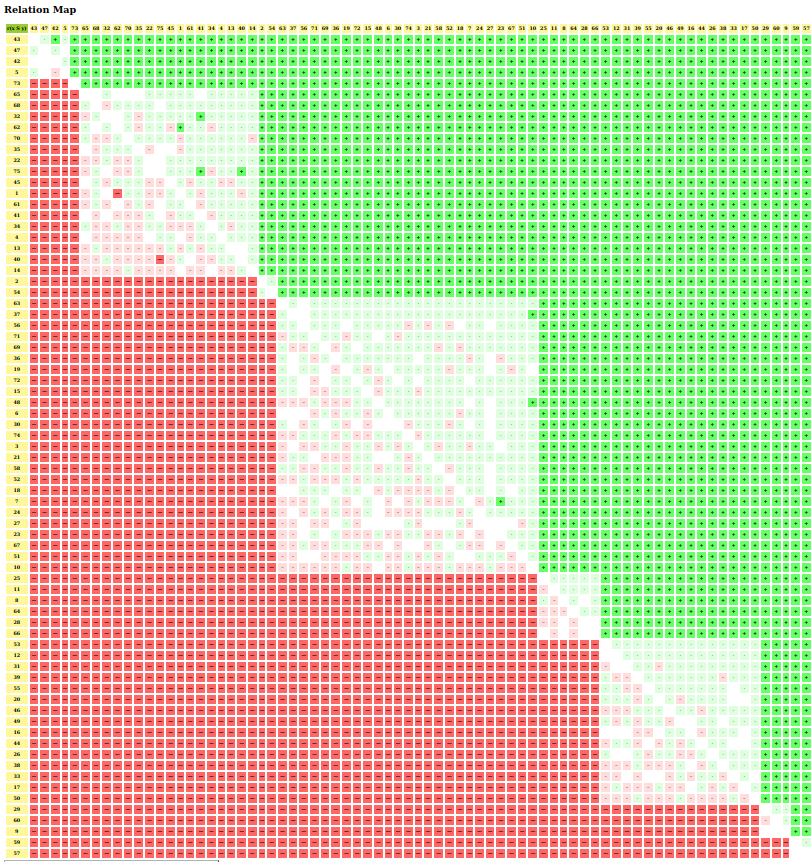
\includegraphics[width=\hsize]{Figures/9-1-sparse75RelationMap.png}
\caption{The relation map of a sparse outranking digraph}
\label{fig:9.1}       % Give a unique label
\end{figure}
%\clearpage

In Fig.~\vref{fig:9.1} we easily recognise the 9 linearly ordered quantile equivalence classes. \emph{Green} and \emph{light-green} pixels show positive \emph{outranking} situations, whereas positive \emph{outranked} --negative outranking-- situations are shown in \emph{red} and \emph{light-red}. Indeterminate situations appear in white. In each one of the 9 quantile equivalence classes we recover the corresponding bipolar-valued outranking \emph{sub-relation}, which leads to an actual \emph{fill-rate} of $20.4\%$ (see List.~\vref{list:9.6} Line~\ref{line:9.6.19}).

Computing the ordinal correlation between the sparse and the standard outranking digraph allows to check how faithful the sparse model represents the complete outranking relation.
\begin{lstlisting}
>>> g = BipolarOutrankingDigraph(tp)
>>> corr = prg.computeOrdinalCorrelation(g)
>>> g.showCorrelation(corr)
  Correlation indexes:
   Crisp ordinal correlation  : +0.863
   Epistemic determination    :  0.315
   Bipolar-valued equivalence : +0.272
\end{lstlisting}   

The ordinal correlation index between the standard and the sparse outranking digraphs is quite high ($+0.863$) and their bipolar-valued equivalence is supported by a mean criteria significance majority of $(1.0+0.272)/2 = 64\%$.

It is worthwhile noticing in Listing~\vref{list:9.6} (Lines~\ref{line:9.6.20} and following) that sparse pre-ranked outranking digraphs do not contain a \texttt{relation} attribute. The access to pairwise outranking characteristic values is here provided via a corresponding \texttt{relation()} function.
\begin{lstlisting}[caption={Functional binary relation characteristics},label=list:9.8]
def relation(self,x,y):
    """
    Dynamic construction of the global
    outranking characteristic function r(x,y).
    """
    Min = self.valuationdomain['min']
    Med = self.valuationdomain['med']
    Max = self.valuationdomain['max']
    if x == y:   §\label{line:9.8.9}§
        return Med  §\label{line:9.8.10}§
    cx = self.actions[x]['component']
    cy = self.actions[y]['component']
    if cx == cy: §\label{line:9.8.13}§
        return self.components[cx]['subGraph'].relation[x][y] §\label{line:9.8.14}§
    elif self.components[cx]['rank'] > self.components[cy]['rank']:
        return Min
    else:
        return Max
\end{lstlisting}

In Listing~\vref{list:9.8} Lines~\ref{line:9.8.9}-\ref{line:9.8.10}, all reflexive situations are set to the \emph{indeterminate} value. When two decision alternatives belong to a same component --quantile equivalence class-- we access the relation attribute of the corresponding outranking sub-digraph (Lines~\ref{line:9.8.13}-\ref{line:9.8.14}). Otherwise we just check the respective ranks of the components.

\section{Ranking pre-ranked sparse outranking digraphs}
\label{sec:9.4}

Each one of these nine ordered components is locally ranked by using a suitable ranking rule. Best operational results, both in run times and quality, are more or less equally obtained with the \Copeland and the \NetFlows rules (see Sect.~\ref{sec:8.2} and Sect.~\ref{sec:8.3}). The eventually obtained linear ordering (from the worst to best) is stored in a \texttt{prg.boostedOrder} attribute. A reversed linear order (from the best to the worst) is stored in a \texttt{prg.boostedRanking} attribute.
  \begin{lstlisting}
>>> prg.boostedRanking
  [43, 47, 42, 5, 73, 65, 68, 32, 62, 70, 35, 22, 75, 45, 1,
   61, 41, 34, 4, 13, 40, 14, 2, 54, 63, 37, 56, 71, 69, 36,
   19, 72, 15, 48, 6, 30, 74, 3, 21, 58, 52, 18, 7, 24, 27,
   23, 67, 51, 10, 25, 11, 8, 64, 28, 66, 53, 12, 31, 39, 55,
   20, 46, 49, 16, 44, 26, 38, 33, 17, 50, 29, 60, 9, 59, 57]
\end{lstlisting}

Alternative \texttt{43} appears \emph{first-ranked}, whereas alternative \texttt{57} is \emph{last-ranked} (see above).

The quality of this ranking result may be assessed by computing with the \texttt{computeRankingCorrelation()} method\index{computeRankingCorrelation@\texttt{computeRankingCorrelation()}} its ordinal correlation index with the standard outranking digraph \texttt{g}.  
\begin{lstlisting}
>>> corr = g.computeRankingCorrelation(prg.boostedRanking)
>>> g.showCorrelation(corr)
 Correlation indexes:
   Crisp ordinal correlation  : +0.807
   Epistemic determination    :  0.315
   Bipolar-valued equivalence : +0.254
\end{lstlisting}

One may also verify below that the \Copeland ranking obtained, for instance, from the standard outranking digraph \texttt{g} is as well highly correlated ($+0.822$) with the one obtained from the sparse outranking digraph \texttt{prg}.
\begin{lstlisting}
   >>> from linearOrders import CopelandOrder
   >>> cop = CopelandOrder(g)
   >>> print(cop.computeRankingCorrelation(prg.boostedRanking))
    {'correlation': 0.822, 'determination': 1.0}
\end{lstlisting}

\vspace{\baselineskip}
Noticing the computational efficiency of the quantiles sorting construction, coupled with the separability property of the quantile class membership characteristics computation, we will make usage of the \texttt{PreRankedOutrankingDigraph} constructor in Chap.~\ref{sec:11} for HPC ranking big and even huge performance tableaux \citep{BIS-2016}. The next Chap.~\ref{sec:10} addresses now the problem of absolute rating into learned quantile performance norms.

%%%%%%% The chapter bibliography
%\normallatexbib
%\clearpage
%\phantomsection
%\addcontentsline{toc}{section}{References}
\chapter{Rating by sorting into relative performance quantiles}
\label{sec:9}

\abstract*{To be written.}

\abstract{To be written.}

We apply order statistics for sorting a set $X$ of $n$ potential decision actions, evaluated on $m$ incommensurable performance criteria, into $q$ quantile equivalence classes, based on pairwise outranking characteristics involving the quantile class limits observed on each criterion. Thus we may implement a weak ordering algorithm of complexity $O(nmq)$.


\section{Quantile sorting on a single criterion}
\label{sec:9.1}

A single criterion sorting category $K$ is a (usually) lower-closed interval $[m_k ; M_k[$ on a real-valued performance measurement scale, with $m_k \leq M_k$. If $x$ is a measured performance on this scale, we may distinguish three sorting situations.
\begin{enumerate}
\item $x < m_k$ and $x < M_k$: The performance $x$ is lower than category $K$.
\item $x \geqslant m_k$ and $x < M_k$: The performance $x$ belongs to category $K$.
\item $x > m_k$ and $x \geqslant M_k$: The performance $x$ is higher than category $K$.
\end{enumerate}

As the relation $<$ is the dual of $\geqslant$ ($\not\geqslant$), it will be sufficient to check that $x \geqslant m_k$ as well as $x \not\geqslant M_k$ are true for $x$ to be considered a member of category $K$.

Upper-closed categories (in a more mathematical integration style) may as well be considered. In this case it is sufficient to check that $m_k \not\geqslant x$ as well as $M_k \geq x$ are true for $x$ to be considered a member of category $K$. It is worthwhile noticing that a category $K$ such that $m_k = M_k$ is hence always empty by definition. In order to be able to properly sort over the complete range of values to be sorted, we will need to use a special, two-sided closed last, respectively first, category.

Let $K = {K_1 , ..., K_q}$ be a non trivial partition of the criterion’s performance measurement scale into $q \geq 2$ ordered categories $K_k$ – i.e. lower-closed intervals $[m_k ; M_k[$ – such that $m_k < M_k$, $M_k = m_{k+1}$ for $k = 0, ..., q - 1$ and $M_q = \infty$. And, let $A=\{a_1 , a_2 , a_3 , ...\}$ be a finite set of not all equal performance measures observed on the scale in question.

\textbf{Property}: For all performance measure $x \in A$ there exists now a unique $k$ such that $x \in K_k$. If we assimilate, like in descriptive statistics, all the measures gathered in a category $K_k$ to the central value of the category – i.e. $(m_k + M_k)/2$ – the sorting result will hence define a weak order (complete preorder) on $A$.

Let $Q=\{Q_0 , Q_1 , ..., Q_q\}$ denote the set of $q + 1$ increasing order-statistical quantiles –like quartiles or deciles– we may compute from the ordered set $A$ of performance measures observed on a performance scale. If $Q_0 = \min(X)$, we may, with the following intervals: $[Q_0 ; Q_1 [$, $[Q_1 ; Q_2 [$, ..., $[Q_{q-1}; \infty[$, hence define a set of $q$ lower-closed sorting categories. And, in the case of upper-closed categories, if $Q_q = \max(X)$, we would obtain the intervals $] -\infty; Q_1]$, $]Q_1 ; Q_2]$, ..., $]Q_{q-1} ; Q_q]$. The corresponding sorting of $A$ will result, in both cases, in a repartition of all measures $x$ into the $q$ quantile categories $K_k$ for $k = 1, ..., q$.

\textbf{Example}: Let $A$ = \{ $a_7 = 7.03$, $a_{15}=9.45$, $a_{11}= 20.35$, $a_{16}= 25.94$, $a_{10}= 31.44$, $a_9= 34.48$, $a_{12}= 34.50$, $a_{13}= 35.61$, $a_{14}= 36.54$, $a_{19}= 42.83$, $a_5= 50.04$, $a_2= 59.85$, $a_{17}= 61.35$, $a_{18}= 61.61$, $a_3= 76.91$, $a_6= 91.39$, $a_1= 91.79$, $a_4= 96.52$, $a_8= 96.56$, $a_{20}= 98.42$ \} be a set of 20 increasing performance measures observed on a given criterion. The lower-closed category limits we obtain with quartiles ($q = 4$) are: $Q_0 = 7.03$ = $a_7$, $Q_1= 34.485$, $Q_2= 54.945$ (median performance), and $Q_3= 91.69$. And the sorting into these four categories defines on $A$ a complete preorder with the following four equivalence classes: $K_1=\{a_7,a_{10},a_{11},a_{10},a_{15},a_{16}\}$, $K_2=\{a_5,a_9,a_{13},a_{14},a_{19}\}$, $K_3=\{a_2,a_3,a_6,a_{17},a_{18}\}$, and $K_4=\{a_1,a_4,a_8,a_{20}\}$.

\section{Quantiles sorting with multiple performance criteria}
\label{sec:9.2}

Let us now suppose that we are given a performance tableau with a set $X$ of $n$ decision alternatives evaluated on a coherent family of $m$ performance criteria associated with the corresponding outranking relation $\succsim$ defined on $X$. We denote $x_j$ the performance of alternative $x$ observed on criterion $j$.

Suppose furthermore that we want to sort the decision alternatives into $q$ upper-closed quantile equivalence classes. We therefore consider a series : $k = k/q$ for $k = 0, ..., q$ of $q+1$ equally spaced quantiles, like quartiles: $0$, $0.25$, $0.5$, $0.75$, $1$; quintiles: $0$, $0.2$, $0.4$, $0.6$, $0.8$, $1$: or deciles: $0$, $0.1$, $0.2$, ..., $0.9$, $1$, for instance.

The upper-closed $\mathbf{q}^k$ class corresponds to the m quantile intervals $]q_j(p_{k-1});q_j(p_k)]$ observed on each criterion $j$,  where $k = 2, ..., q$ , $q_j(p_q) =  \max_X(x_j)$, and the first class gathers all performances below or equal to $Q_j(p_1)$.

The lower-closed $\mathbf{q}_k$ class corresponds to the $m$ quantile intervals $[q_j(p_{k-1});q_j(p_k)[$ observed on each criterion $j$, where $k = 1, ..., q-1$, $q_j(p_0) = \min_X(x_j)$, and the last class gathers all performances above or equal to $Q_j(p_{q-1})$.

We call \textbf{q-tiles} a complete series of $k = 1, ..., q$ upper-closed $\mathbf{q}^k$, respectively lower-closed $\mathbf{q}_k$, multiple criteria quantile classes.

\textbf{Property}: With the help of the bipolar-valued characteristic of the outranking relation $r(\succsim)$ we may compute the bipolar-valued characteristic of the assertion: $x$ belongs to upper-closed *q*-tiles class $\mathbf{q}^k$ class, resp. lower-closed class $\mathbf{q}_k$, as follows:
\begin{eqnarray}
r(x \in \mathbf{q}^k) \; = \; \min \big[ -r\big(\mathbf{q}(p_{q-1}) \succsim x\big), \,r\big(\mathbf{q}(p_{q}) \succsim x)\big]\\
r(x \in \mathbf{q}_k) \; = \; \min \big[ r\big(x \succsim \mathbf{q}(p_{q-1})\big),\, -r\big(x \succsim\mathbf{q}(p_{q})\big)\big]
\end{eqnarray}

The outranking relation $\succsim$ verifying the coduality principle, $-r\big(\mathbf{q}(p_{q-1}) \succsim x\big) \,=\, r\big(\mathbf{q}(p_{q-1}) \prec x\big)$, resp. $-r\big(x \succsim \mathbf{q}(p_{q}) \,=\, r\big(x \prec \mathbf{q}(p_{q}\big)$.

We may compute, for instance, a five-tiling of a given random performance tableau with the help of the \texttt{QuantilesSortingDigraph} class.

\begin{lstlisting}[caption={Computing a quintiles sorting result},label=list:9.1]
>>> from randomPerfTabs import RandomPerformanceTableau
>>> t = RandomPerformanceTableau(numberOfActions=50,seed=5)
>>> from sortingDigraphs import QuantilesSortingDigraph
>>> qs = QuantilesSortingDigraph(t,limitingQuantiles=5)
>>> qs
    *-----  Object instance description -----------*
     Instance class  : QuantilesSortingDigraph
     Instance name   : sorting_with_5-tile_limits
     # Actions       : 50
     # Criteria      : 7
     # Categories    : 5
     Lowerclosed     : False
     Size            : 841
     Valuation domain  : [-1.00;1.00]
     Determinateness (%) : 81.39
     Attributes          : ['actions','actionsOrig',
          'criteria','evaluation','runTimes','name',
	  'limitingQuantiles','LowerClosed',
	  'categories','criteriaCategoryLimits',
	  'profiles','profileLimits','hasNoVeto',
	  'valuationdomain','nbrThreads','relation',
	  'categoryContent','order','gamma','notGamma']
     *------  Constructor run times (in sec.) ------*
     # Threads        : 1
     Total time       : 0.03120
     Data input       : 0.00300
     Compute profiles : 0.00075
     Compute relation : 0.02581
     Weak Ordering    : 0.00052
     
>>> qs.showCriteriaQuantileLimits()
     Quantile Class Limits (q = 5)
     Upper-closed classes
     crit.	 0.20	 0.40	 0.60	 0.80	 1.00	 
     *------------------------------------------------
      g1	 31.35	 41.09	 58.53	 71.91	 98.08	 
      g2	 27.81	 39.19	 49.87	 61.66	 96.18	 
      g3	 25.10	 34.78	 49.45	 63.97	 92.59	 
      g4	 24.61	 37.91	 53.91	 71.02	 89.84	 
      g5	 26.94	 36.43	 52.16	 72.52	 96.25	 
      g6	 23.94	 44.06	 54.92	 67.34	 95.97	 
      g7	 30.94	 47.40	 55.46	 69.04	 97.10	 

>>> qs.showSorting()
    *--- Sorting results in descending order ---*
     ]0.80 - 1.00]: ['a22']
     ]0.60 - 0.80]: ['a03','a07','a08','a11','a14','a17',
                     'a19','a20','a29','a32','a33','a37',
		     'a39','a41','a42','a49']
     ]0.40 - 0.60]: ['a01','a02','a04','a05','a06','a08',
                     'a09','a16','a17','a18','a19','a21',
		     'a24','a27','a28','a30','a31','a35',
		     'a36','a40','a43','a46','a47','a48',
		     'a49','a50']
     ]0.20 - 0.40]: ['a04','a10','a12','a13','a15','a23',
                     'a25','a26','a34','a38','a43','a44',
		     'a45','a49']
     ]   < - 0.20]: ['a44']
   \end{lstlisting}
   
Most of the decision actions (26) are gathered in the median quintile $]0.40 - 0.60]$ class, whereas the highest quintile $]0.80-1.00]$ and the lowest quintile $]< - 0.20]$ classes gather each one a unique decision alternative ($a22$, resp. $a44$) (see Listing \ref{list:9.1} Lines 45-).

We may inspect as follows the details of the corresponding sorting characteristics.

\begin{lstlisting}[caption={Bipolar-valued sorting characteristics (extract)},label=list:9.2]
>>> qs.valuationdomain
    {'min': Decimal('-1.0'), 'med': Decimal('0'),
     'max': Decimal('1.0')}
>>> qs.showSortingCharacteristics()
     x  in  q^k          r(q^k-1 < x)  r(q^k >= x)  r(x in q^k)
    a22 in ]< - 0.20]	    1.00	 -0.86	      -0.86
    a22 in ]0.20 - 0.40]    0.86	 -0.71	      -0.71
    a22 in ]0.40 - 0.60]    0.71	 -0.71	      -0.71
    a22 in ]0.60 - 0.80]    0.71	 -0.14	      -0.14
    a22 in ]0.80 - 1.00]    0.14	  1.00	       0.14
    ...
    ...
    a44 in ]< - 0.20]	    1.00	  0.00	       0.00
    a44 in ]0.20 - 0.40]    0.00	  0.57	       0.00
    a44 in ]0.40 - 0.60]   -0.57	  0.86	      -0.57
    a44 in ]0.60 - 0.80]   -0.86	  0.86	      -0.86
    a44 in ]0.80 - 1.00]   -0.86	  0.86	      -0.86
    ...
    ...
    a49 in ]< - 0.20]	    1.00	 -0.43	      -0.43
    a49 in ]0.20 - 0.40]    0.43	  0.00	       0.00
    a49 in ]0.40 - 0.60]    0.00	  0.00	       0.00
    a49 in ]0.60 - 0.80]    0.00	  0.57	       0.00
    a49 in ]0.80 - 1.00]   -0.57	  0.86	      -0.57
\end{lstlisting}
  
Alternative $a22$ verifies indeed positively both sorting conditions only for the highest quintile $[0.80 - 1.00]$ class (see Listing \ref{list:9.2} Lines 10). Whereas alternatives $a44$ and $a49$, for instance, weakly verify both sorting conditions each one for two, resp. three, adjacent quintile classes (see Lines 13-14 and 21-23).  

Quantiles sorting results indeed always verify the following \textbf{Properties}.
\begin{enumerate}
\item \textbf{Coherence}: Each object is sorted into a non-empty subset of \emph{adjacent} $q$-tiles classes. An alternative that would \emph{miss} evaluations on all the criteria will be sorted conjointly in all $q$-tiled classes.
\item \textbf{Uniqueness}: If $r(x \in \mathbf{q}^k) \neq 0$  for $k = 1, ..., q$, then performance $x$ is sorted into \emph{exactly one single} $q$-tiled class.
\item \textbf{Separability}: Computing the sorting result for performance $x$ is independent from the computing of the other performances’ sorting results. This property gives access to efficient parallel processing of class membership characteristics.
\end{enumerate}

The $q$-tiles sorting result leaves us hence with more or less \emph{overlapping} ordered quantile equivalence classes. For constructing now a linearly ranked q-tiles partition of $X$ , we may apply three strategies:
\begin{enumerate}
\item \textbf{Average} (default): In decreasing lexicographic order of the average of the lower and upper quantile limits and the upper quantile class limit;
\item \textbf{Optimistic}: In decreasing lexicographic order of the upper and lower quantile class limits;
\item \textbf{Pessimistic}: In decreasing lexicographic order of the lower and upper quantile class limits;
\end{enumerate}

\begin{lstlisting}[caption={Weakly ranking the quintiles sorting result},label=list:9.3]
>>> qs.showQuantileOrdering(strategy='average')
    ]0.80-1.00] : ['a22']
    ]0.60-0.80] : ['a03','a07','a11','a14','a20','a29',
                   'a32','a33','a37','a39','a41','a42']
    ]0.40-0.80] : ['a08','a17','a19']
    ]0.20-0.80] : ['a49']
    ]0.40-0.60] : ['a01','a02','a05','a06','a09','a16',
                    'a18','a21','a24','a27','a28','a30',
		    'a31','a35','a36','a40','a46','a47',
		    'a48','a50']
    ]0.20-0.60] : ['a04','a43']
    ]0.20-0.40] : ['a10','a12','a13','a15','a23','a25',
                    'a26','a34','a38','a45']
    ]  < -0.40] : ['a44']
\end{lstlisting}

Following, for instance, the \emph{average} ranking strategy, we find confirmed in the weak ranking shown in Listing \ref{list:9.3},  that alternative $a49$  is indeed sorted into three adjacent quintiles classes, namely $]0.20-0.80]$ (see Line 6) and precedes the $]0.40-0.60]$ class, of same average of lower and upper limits.

The \texttt{QuantilesSortingDigraph} constructor gives hence a linearly ordered decomposition of the corresponding bipolar-valued outranking digraph. This decomposition leads us to a new \textbf{sparse pre-ranked} outranking digraph model.

\section{The sparse pre-ranked outranking digraph model}
\label{sec:9.3}

We may notice that a given outranking digraph -the association of a set of decision alternatives and an outranking relation- is, following the methodological requirements of the outranking approach, necessarily associated with a corresponding performance tableau. And, we may use this underlying performance tableau for linearly decomposing the set of potential decision alternatives into ordered quantiles equivalence classes by using the quantiles sorting technique seen in the previous Section. 

In the coding example shown in Listing \ref{list:9.4} below, we generate for instance, first (Lines 2-3), a simple performance tableau of 75 decision alternatives and, secondly (Lines 4-6), we construct the corresponding \texttt{PreRankedOutrankingDigraph} instance called $prg$. Notice by the way the \texttt{BigData} flag (Line 3) used here for generating a parsimoniously commented performance tableau.

\begin{lstlisting}[caption={Computing a \emph{pre-ranked} sparse outranking digraph},label=list:9.4]
>>> from randomPerfTabs import RandomPerformanceTableau
>>> tp = RandomPerformanceTableau(numberOfActions=75,\
...                               BigData=True,seed=100)
>>> from sparseOutrankingDigraphs import\
...          PreRankedOutrankingDigraph
>>> prg = PreRankedOutrankingDigraph(Tp,quantiles=5)
>>> prg
    *----- Object instance description ------*
     Instance class    : PreRankedOutrankingDigraph
     Instance name     : randomperftab_pr
     Actions           : 75
     Criteria          : 7
     Sorting by        : 5-Tiling
     Ordering strategy : average
     Components        : 9
     Minimal order     : 1
     Maximal order     : 25
     Average order     : 8.3
     fill rate         : 20.432%
     Attributes        : ['actions','criteria','evaluation','NA','name',
         'order','runTimes','dimension','sortingParameters',
	 'valuationdomain','profiles','categories','sorting',
	 'decomposition','nbrComponents','components',
	 'fillRate','minimalComponentSize','maximalComponentSize', ... ]
\end{lstlisting}

The ordering of the 5-tiling result is following the \emph{average} lower and upper quintile limits strategy (see Listing \ref{list:9.4} Line 14). We obtain here 9 ordered components of minimal order 1 and maximal order 25. The corresponding \emph{pre-ranked decomposition} may be visualized as follows.

\begin{lstlisting}[caption={The quantiles decomposition of a pre-ranked outranking digraph},label=list:9.5]
>>> prg.showDecomposition()
    *--- quantiles decomposition in decreasing order---*
     c1. ]0.80-1.00] : [5, 42, 43, 47]
     c2. ]0.60-1.00] : [73]
     c3. ]0.60-0.80] : [1, 4, 13, 14, 22, 32, 34, 35, 40,
                        41, 45, 61, 62, 65, 68, 70, 75]
     c4. ]0.40-0.80] : [2, 54]
     c5. ]0.40-0.60] : [3, 6, 7, 10, 15, 18, 19, 21, 23, 24,
                        27, 30, 36, 37, 48, 51, 52, 56, 58,
			63, 67, 69, 71, 72, 74]
     c6. ]0.20-0.60] : [8, 11, 25, 28, 64, 66]
     c7. ]0.20-0.40] : [12, 16, 17, 20, 26, 31, 33, 38, 39,
                        44, 46, 49, 50, 53, 55]
     c8. ]   <-0.40] : [9, 29, 60]
     c9. ]   <-0.20] : [57, 59]
\end{lstlisting}

The highest quintile class ($]80\%-100\%]$) contains decision alternatives 5, 42, 43 and 47. Lowest quintile class ($]-20\%]$) gathers alternatives 57 and 59 (see Listing \ref{list:9.5} Lines 3 and 15). We may inspect the resulting sparse outranking relation map as follows in a browser view.

\begin{lstlisting}
   >>> prg.showHTMLRelationMap()
\end{lstlisting}

\begin{figure}[h]
%\sidecaption
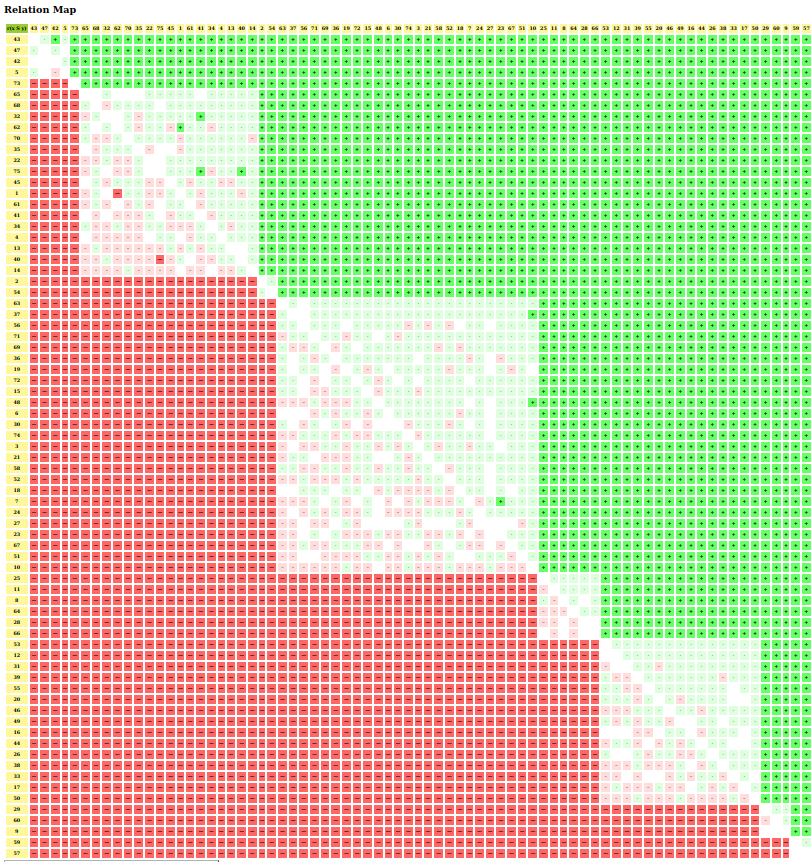
\includegraphics[width=9cm]{Figures/sparse75RelationMap.png}
\caption{The relation map of a sparse outranking digraph.}
\label{fig:9.1}       % Give a unique label
\end{figure}
\clearpage
In Fig. \ref{fig:9.1} we easily recognize the 9 linearly ordered quantile equivalence classes. \emph{Green} and \emph{light-green} show positive \textbf{outranking} situations, whereas positive \textbf{outranked} situations are shown in \emph{red} and \emph{light-red}. Indeterminate situations appear in white. In each one of the 9 quantile equivalence classes we recover in fact the corresponding bipolar-valued outranking \emph{sub-relation}, which leads to an actual \textbf{fill-rate} of $20.4\%$ (see Listing \ref{list:9.4} Line 19).

We may now check how faithful the sparse model represents the complete outranking relation.

\begin{lstlisting}
   >>> g = BipolarOutrankingDigraph(tp)
   >>> corr = prg.computeOrdinalCorrelation(g)
   >>> g.showCorrelation(corr)
    Correlation indexes:
     Crisp ordinal correlation  : +0.863
     Epistemic determination    :  0.315
     Bipolar-valued equivalence : +0.272
\end{lstlisting}   

The ordinal correlation index between the standard and the sparse outranking relations is quite high ($+0.863$) and their bipolar-valued equivalence is supported by a mean criteria significance majority of $(1.0+0.272)/2 = 64\%$.

It is worthwhile noticing in Listing \ref{list:9.4} Lines 20- that sparse pre-ranked outranking digraphs do not contain a \texttt{relation} attribute. The access to pairwise outranking characteristic values is here provided via a corresponding \texttt{relation()} function.

\begin{lstlisting}
def relation(self,x,y):
    """
    Dynamic construction of the global
    outranking characteristic function r(x,y).
    """
    Min = self.valuationdomain['min']
    Med = self.valuationdomain['med']
    Max = self.valuationdomain['max']
    if x == y:
        return Med
    cx = self.actions[x]['component']
    cy = self.actions[y]['component']
    if cx == cy:
        return self.components[cx]['subGraph'].relation[x][y]
    elif self.components[cx]['rank'] > self.components[cy]['rank']:
        return Min
    else:
        return Max
\end{lstlisting}

All reflexive situations are set to the \emph{indeterminate} value. When two decision alternatives belong to a same component -quantile equivalence class- we access the relation attribute of the corresponding outranking sub-digraph. Otherwise we just check the respective ranks of the components.

\section{Ranking pre-ranked sparse outranking digraphs}
\label{sec:9.4}

Each one of these 9 ordered components may now be locally ranked by using a suitable ranking rule. Best operational results, both in run times and quality, are more or less equally given with the \Copeland and the \NetFlows rules. The eventually obtained linear ordering (from the worst to best) is stored in a \texttt{prg.boostedOrder} attribute. A reversed linear ranking (from the best to the worst) is stored in a \texttt{prg.boostedRanking} attribute.
  
\begin{lstlisting}
>>> prg.boostedRanking
  [43, 47, 42, 5, 73, 65, 68, 32, 62, 70, 35, 22, 75, 45, 1,
   61, 41, 34, 4, 13, 40, 14, 2, 54, 63, 37, 56, 71, 69, 36,
   19, 72, 15, 48, 6, 30, 74, 3, 21, 58, 52, 18, 7, 24, 27,
   23, 67, 51, 10, 25, 11, 8, 64, 28, 66, 53, 12, 31, 39, 55,
   20, 46, 49, 16, 44, 26, 38, 33, 17, 50, 29, 60, 9, 59, 57]
\end{lstlisting}

Alternative 43 appears \emph{first ranked}, whereas alternative 57 is \emph{last ranked} (see Line 2 and 6 above). The quality of this ranking result may be assessed by computing its ordinal correlation with the standard outranking relation.  

\begin{lstlisting}
>>> corr = g.computeRankingCorrelation(prg.boostedRanking)
>>> g.showCorrelation(corr)
 Correlation indexes:
   Crisp ordinal correlation  : +0.807
   Epistemic determination    :  0.315
   Bipolar-valued equivalence : +0.254
\end{lstlisting}

We may also verify below that the \Copeland ranking obtained from the standard outranking digraph is highly correlated ($+0.822$) with the one obtained from the sparse outranking digraph.

\begin{lstlisting}
   >>> from linearOrders import CopelandOrder
   >>> cop = CopelandOrder(g)
   >>> print(cop.computeRankingCorrelation(prg.boostedRanking))
    {'correlation': 0.822, 'determination': 1.0}
\end{lstlisting}

Noticing the computational efficiency of the quantiles sorting construction, coupled with the separability property of the quantile class membership characteristics computation, we will make usage of the \texttt{PreRankedOutrankingDigraph} constructor for HPC ranking big and even huge performance tableaux (see Chapter \ref{sec:11}).
 

%\bibliographystyle{spbasic}
%\bibliography{03-backMatters/reference}
 
